\documentclass{beamer}

\usepackage{enumerate}
\usepackage[utf8x]{inputenc}
%\usepackage{default}
\usepackage{hyperref}
\usepackage{graphicx,wasysym}
\usepackage{subfigure}
\usepackage{fixltx2e}%for subscript superscript
\usepackage{amsmath}
\usepackage{amsfonts}
\usepackage{setspace}
\usepackage{xcolor}
\usepackage{algorithmic}
\usepackage{caption}
%\usepackage[lined,boxed]{algorithm2e}
%\usepackage[linesnumbered,vlined,portugues]{algorithm2e} 



% latex

% Related to VCD

\newcommand{\VC}{\textrm{\sf VC}}
\newcommand{\SVC}{\textrm{\sf SVC}}
\newcommand{\negs}{\textrm{\sf negs}}
\newcommand{\VCDimC}{\textrm{\sf VCD}}
\newcommand{\SVCDimC}{\textrm{\sf SVCD}}
\newcommand{\vcd}{\textrm{{\sf VC}-dimension}}
\newcommand{\svcd}{\textrm{Subspace {\sf VC}-dimension}}

\newcommand{\Th}{\textrm{\sc Th}}

% Complexity Classes
\newcommand{\UNSAT}{\textrm{\sf UNSAT}}
\newcommand{\SAT}{\textrm{\sf SAT}}
% Fourier symbols
\newcommand{\wt}[1]{\widetilde{#1}}
\newcommand{\wh}[1]{\widehat{#1}}
\newcommand{\sse}{\subseteq}
\newcommand{\bits}{\{-1,1\}}
\newcommand{\zo}{\{0,1\}}
\newcommand{\bn}{\bits^n}
\newcommand{\zon}{\zo^n}
\newcommand{\isafunc}{:\bn\to\bits}
\newcommand{\isazofunc}{:\zo^n\to\zo}
\newcommand{\sumi}{\sum_{i=1}^n}
\newcommand{\cond}{\,|\,}
\newcommand{\defn}{\stackrel{\text{\tiny def}}{=}}
\newcommand{\zap}[1]{}
\newcommand{\ind}{\mathsf{Ind} }
\newcommand{\cpm}{C_{\oplus,\min}}
\newcommand{\degtwo}{\mathsf{deg_{\F_2}}}
\newcommand{\fhat}{\widehat{f}}
\newcommand{\ghat}{\widehat{g}}
\newcommand{\pmo}{\set{-1,1}}
\newcommand{\pmon}{\pmo^n}
\newcommand{\I}{\mathbf{I}}
\newcommand{\sps}{\mathsf{sparsity}}
\newcommand{\fdim}{\mathsf{fdim}}
\newcommand{\gr}{\mathsf{gr}}

% left-right wrappers
\newcommand{\card}[1]{\left | \set{#1}\right |}
\newcommand{\set}[1]{\left\{ #1 \right\}}
\newcommand{\cset}[1]{\left ( #1 \right )}
\newcommand{\abs}[1]{\left\lvert #1 \right\rvert}
%\newcommand{\norm}[1]{\left\lVert #1 \right\rVert}
\newcommand{\floor}[1]{\left\lfloor #1 \right\rfloor}
\newcommand{\ceil}[1]{\left\lceil #1 \right\rceil}

% latin
\newcommand{\etal}{\textit{et al}.\@\xspace}
\newcommand{\ie}{i.e.}

% models
\newcommand{\CREW}{\textsf{CREW}}
\newcommand{\DT}{\mathsf{DT}}

% Boolean function parameters
\newcommand{\sens}{\mathsf{s}}
\newcommand{\tsens}{\mathsf{ts}}
\newcommand{\bsens}{\mathsf{bs}}
\newcommand{\cert}{\mathsf{C}}
\newcommand{\altr}{\mathsf{alt}}
\newcommand{\salt}{\mathsf{salt}}
\renewcommand{\deg}{\mathsf{deg}}
\newcommand{\inv}{\mathtt{I}}
\newcommand{\indim}{\mathtt{indim}}
\newcommand{\outdim}{\mathtt{outdim}}


% short hands
\newcommand{\lep}{\preccurlyeq}
\newcommand{\pgeq}{\succcurlyeq}
\newcommand{\calA}{{\cal A}}
\newcommand{\calB}{{\cal B}}
\newcommand{\calC}{{\cal C}}
\newcommand{\calD}{{\cal D}}
\newcommand{\calE}{{\cal E}}
\newcommand{\calF}{{\cal F}}
\newcommand{\calG}{{\cal G}}
\newcommand{\calH}{{\cal H}}
\newcommand{\calI}{{\cal I}}
\newcommand{\calJ}{{\cal J}}
\newcommand{\calK}{{\cal K}}
\newcommand{\calL}{{\cal L}}
\newcommand{\calM}{{\cal M}}
\newcommand{\calN}{{\cal N}}
\newcommand{\calO}{{\cal O}}
\newcommand{\calP}{{\cal P}}
\newcommand{\calQ}{{\cal Q}}
\newcommand{\calR}{{\cal R}}
\newcommand{\calS}{{\cal S}}
\newcommand{\calT}{{\cal T}}
\newcommand{\calU}{{\cal U}}
\newcommand{\calV}{{\cal V}}
\newcommand{\calW}{{\cal W}}
\newcommand{\calX}{{\cal X}}
\newcommand{\calY}{{\cal Y}}
\newcommand{\calZ}{{\cal Z}}


% bold math : for probabiliy
\newcommand{\bldS}{\mathbf{S}}
\newcommand{\bldx}{\mathbf{x}}
\newcommand{\bldX}{\mathbf{X}}
\newcommand{\bldsbar}{\mathbf{\overline{s}}}


% Boolean functions.
\newcommand{\DISJ}{\mbox{\sf DISJ}}
\newcommand{\SDISJ}{\mbox{\sf SDISJ}}
\newcommand{\INEQ}{\mbox{\sf INEQ}}
\newcommand{\PDISJ}{\mbox{\sf PDISJ}}
%\newcommand{\AND}{\wedge}
%\newcommand{\OR}{\vee}
\newcommand{\sat}{\textrm{\bf SAT}}
\newcommand{\match}{\mbox{\sf MATCH}}
\newcommand{\MAJ}{\mathsf{MAJ}}
\newcommand{\ANDOR}{\mathop{\mbox{$\mathsf{AND}$-$\mathsf{OR}$}}}
\newcommand{\ADDR}{\mathsf{ADDR}}

% math symbols
\newcommand{\expct}[1]{\mathbb{E}\left[ #1 \right]}
\newcommand{\gaussian}[3]{ {#1 \brack #2}_{#3}}

% communication complexity
\newcommand{\CC}{\mathsf{CC}}


% fields
\newcommand{\field}{\mathbb{F}}
\newcommand{\F}{{\mathbb{F}}}
\newcommand{\Q}{{\mathbb{Q}}}
\newcommand{\N}{{\mathbb{N}}}
\newcommand{\R}{{\mathbb{R}}}

% linear algebra
\newcommand{\rank}[1]{\mathsf{rank} \left( #1 \right)}
\newcommand{\rspace}[1]{\mathsf{rowspace} \left( #1 \right)}
%\newcommand{\degtwo}{\mathsf{deg_{\F_2}}}
\renewcommand{\deg}{\mathsf{deg}}


\usetheme{Boadilla} % Taken from Overleaf
\graphicspath{ {./images/} }

%\usetheme{Berlin} %writes content horizontally on top
%\setbeamertemplate{page number in head/foot}[totalframenumber] %gives slide number
\setbeamertemplate{itemize item}[triangle]




\setbeamercolor{title}{fg=red!40!black}
%\setbeamercolor{title}{fg=red!40!black,bg=green!40!white}

\title{ \sc \color{blue}{Chordal graphs are easily testable}}
\subtitle{Rémi de Joannis de Verclos}
\author{Presented by - Amit Roy  }
\institute{Spring School 2025}
% NUS - \date{August 21,  2023}
\date{May 14, 2025}



\begin{document}
 
\begin{frame}
\titlepage
\end{frame} 



\section{Introduction}

\begin{frame}
	
\includegraphics[scale=0.4]{graph-property-testing}
\end{frame}

\begin{frame}{Graph Property Testing}
	
	\begin{block}{Graph Property}
		
	A {\bf graph property} is a set of graphs that is closed under graph
	isomorphism. That is, $\Pi$ is a graph property if, for every graph $G = (V, E)$ and every bijection
	$\pi : V \to V '$, it holds that $G \in \Pi$ if and only if $\pi(G) \in\Pi$, where $\pi(G)$ is the graph obtained from $G$
	by relabelling the vertices according to $\pi$; that is,
	$$\pi(G) = (V', {{\pi(u),\pi(v)} \mid \{u,v\} \in E} )$$
	\end{block}


	
\end{frame}


\begin{frame}{Definition}
	\begin{block}{$\epsilon$-far from property $\calP$}
	A graph $G$ on $n$ vertices is $\epsilon$-far from satisfying a property $\mathcal{P}$ if one has to add
	or delete at least $\epsilon n^2$ edges to $G$ to obtain a graph satisfying $\mathcal{P}$.
	\end{block}
\end{frame}

\begin{frame}{Definition}
	\begin{block}{$\epsilon$-tester}
An algorithm $\calA$ is an $\epsilon$-tester for property $\calP$ if it
		\begin{enumerate}
			\item accepts all $x \in \calP$ with probability at least $2/3$	and
			\item  rejects all $x$ that are $\epsilon$-far from $\calP$ with probability at least $2/3$
		\end{enumerate}
		where the probability is taken over the internal coin tosses of $\calA$.
	\end{block}
\pause
\begin{itemize}
	\item The tester has one-sided error if it always accepts functions satisfying $\calP$.
	\pause
	\item  If the queries made by the algorithm do not depend on the answers to the previous queries, $\calA$ is called a {\em nonadaptive} tester.
	Otherwise, it is an {\em adaptive} tester.
\end{itemize}

\end{frame}

\begin{frame}{Definition}
	A hereditary class $\calP$ of graphs is testable if for every fixed $\epsilon > 0$ there is a size $m_{\epsilon}$ such that the following holds. \pause
	\begin{itemize}
		\item If G is $\epsilon$-far from $\calP$ then a set $ X \subseteq V (G)$ sampled
		uniformly at random among all subsets of $V (G)$ of size $m_{\epsilon}$ induces a graph $G[X]$
		that is not in $\calP$ with probability at least $2/3$. \pause
		\item  The property $\calP$ is easily testable if
		moreover $m_{\epsilon}$ is a polynomial function of $\frac{1}{\epsilon}$. Otherwise, $\calP$ is hard to test.
	\end{itemize}

\end{frame}


\begin{frame}
	\begin{center}
		
\includegraphics[scale=0.6]{motivation}
	\end{center}
	
\end{frame}

\begin{frame}{Motivation}
	\begin{itemize}
		
	\item Need to efficiently analyze large graphs using algorithms that provide approximate answers with minimal computational resources 
	 \pause
	\item Property testing allows decisions based on a sublinear number of queries (e.g., inspecting only a random subset of edges or vertices)
	\pause
	\item  For example, testing whether a graph is bipartite can be done without examining all edges.
	\pause
	\item Testers can act as a fast preliminary check to avoid running slower exact algorithms on graphs far from the desired property 
\end{itemize}
\end{frame}


\begin{frame}
	\begin{center}
		
\includegraphics[scale=0.5]{previous-works}
	\end{center}
	
\end{frame}

\begin{frame}{Previous Works}
	\begin{itemize}
		\item Every hereditary property has a one-sided tester [Alon and Shapira 2008]. \pause
		\item {\em Query complexity} - tower of towers of exponentials of size polynomial in $\epsilon ^{-1}$ \pause
		\item Alon and Shapira also showed that class $H$-{ FREE} of graphs without induced copy of $H$ is hard to test when $H$ is different from $P_2, P_3, P_4, C_4$ and different from complement of one of these graphs.
		\pause
		\item This class is known to be easily testable when  $H \in \set{P_2, P_3, P_4}$ . \pause
		\item $H$ for which the class $H$-free is easily testable are known except when $H$ is $C_4$ or its complement $C_4= 2K_2$.
	\end{itemize}
\end{frame}

\begin{frame}{Previous Works}
	\begin{center}
	
		\alert{ \huge Is $C_4$-FREE easily testable?}
	\end{center}
\pause
\begin{block}{Gishboliner and Shapira 2018}
	Every graph that is $\epsilon$-far  from being $C_4$-FREE  contains at least $\frac{n^4}{2^{(1/\epsilon)^c}}$ induced copies of $C_4$ for some constant $c$, implying $C_4$-FREE  can be tested with query complexity $2^{(1/\epsilon)^c}$.
\end{block}
\end{frame}

\begin{frame}{This Paper}
	
	\begin{block}{Chordal Graphs}
		A graph $G$ is chordal if it does not contain any induced cycle of length at least four; i.e., any $(\ge 4)$-cycle in $G$ has a chord (an edge between non-consecutive vertices of the cycle).
	\end{block}
	\pause
	\begin{itemize}
		\item Chordal graphs is an important and natural subclass of $C_4$-FREE. \pause
		\item From Gishboliner and Shapira's work, this class is testable with query complexity $2^{(1/\epsilon)^c}$. \pause
		\item They also conjectured that this bound can be further improved to a polynomial in $\frac{1}{\epsilon}$.
	\end{itemize}

\end{frame}

\begin{frame}{This Paper}
	\begin{itemize}
		\item {\bf The class of chordal graph is easily testable.}
	\end{itemize}
	\begin{block}{Theorem}
		The class of chordal graph is testable with query complexity $\calO(\epsilon ^{-37})$.
	\end{block}
	
\end{frame}

\begin{frame}{Testing Connectedness}
	
	{\bf Input} : A graph $G = (V, E)$ of degree at most $d$, represented by adjacency lists. \\
	\pause
	 {\bf Goal } : An $\epsilon$-tester for connectedness (that accepts all connected graphs with probability $\ge 2/3$
	 , and
	rejects with probability$\ge 2/3$ all graphs that are $\epsilon$-far from connected. \\
	\pause
	{\bf Idea} :  Graphs that are far from connected have many connected components, and therefore they also
	have many ``small" connected components.
\end{frame}

\begin{frame}{Testing Connectedness}
	
	
	{\bf Algorithm}
	
	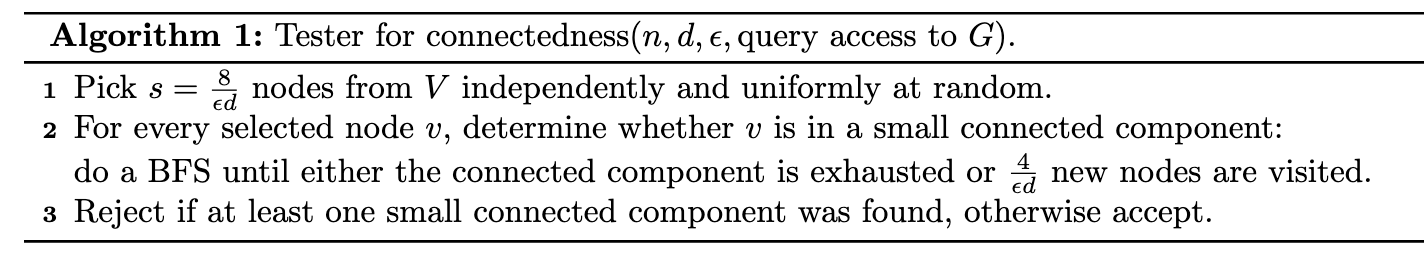
\includegraphics[scale=0.5]{connect-algo}
	\pause
	\begin{itemize}
		\item {\bf Query Complexity } -  $\calO(\frac{1}{\epsilon ^ 2 d})$
		\item Running Time - same
		
	\end{itemize}
	
\end{frame}

\begin{frame}{Proof}
 	\begin{exampleblock}{Claim 1}
 		If G is $\epsilon$-far from connected, it has at least $\frac{\epsilon d n}{2}$ connected components.
 	\end{exampleblock}
 \pause
 	\begin{exampleblock}{Claim 2}
 		If G is $\epsilon$-far from connected, it has at least $\frac{\epsilon dn}{4}$ connected components of size at most $\frac{4}{\epsilon d}$.
 \end{exampleblock}

\pause
{\bf Proof of Query Complexity}:
\begin{itemize}
	\item From Claim 2 we have, at least $\frac{\epsilon d n}{4}$ nodes are in small connected components (of size $\le \frac{4}{\epsilon d}$). 
	\item At least $\frac{\epsilon d}{4}$ fraction of the nodes of the graph "witness" that it is not connected.
	\item It suffices to look at $\frac{2}{\epsilon d /4} = \frac{8}{\epsilon d}$ random samples to get at least one witness with probability  $\ge \frac{2}{3}$.
\end{itemize}

\end{frame}


\begin{frame}{Chordal Graphs}
	
	{\bf Algorithm:}
	\begin{enumerate}
		\item Sample a set of $s=\calO(\epsilon^{-37})$ vertices  $X$ u.a.r. 
		\item If $G[X]$ is chordal then Return ``YES"
		\item Else Return ``NO"
	\end{enumerate}
\pause
\vspace{1cm}
\begin{itemize}
	\item {\bf Query Complexity} - $\calO(\epsilon^{-37})$
	\item {\bf Time Complexity} - $poly(\epsilon^{-37}))$
\end{itemize}
\end{frame}

\begin{frame}{Chordal Graphs}
	
	{\bf Properties}
	\begin{itemize}
		\item A vertex of a graph is {\it simplicial} if its neighbourhood is a clique. \pause
		\item Chordal graphs are stable by addition of simplicial vertices.
		\item Chordal graphs are exactly the graphs that can be obtained from the empty graph by iteratively adding simplicial vertices.
	\end{itemize}
\pause
\begin{exampleblock}{}
	For a vertex $v$ of a graph $G$, let $p_G(v)$ be the number of non-edges in the neighborhood of $v$. 
\end{exampleblock}
\pause
\begin{itemize}
	\item $v$ is simplicial if and only if $p_G(v) = 0$.
\end{itemize}

\end{frame}

\begin{frame}{Nearly Simplicial Vertices}
	\begin{alertblock}{Theorem}
		Let $\epsilon > 0$ and $n \ge \epsilon ^ {-1}$. Let $G$ be a graph with  vertex partition $X \cup Y$ such that $G[Y]$ is chordal and $p_G(v) \le \epsilon n^2$ for every $v \in X$. Then $G$ is $6\epsilon ^ {1/2}$-close from a chordal graph.
	\end{alertblock}
\end{frame}



\begin{frame}{Main Theorem - Proof Overview}
	
	
	{\bf Bird's View}
	
	\begin{enumerate}
		\item Use the {\em Simplicial }Theorem, with a parameter $\delta$ such that $6\delta ^{1/2} = \frac{\epsilon}{2} $.
		\item Partition the vertex set into two sets (vertices whose neighborhoods have few non-edges) and Y (the rest).
		\item Using testability of k-coloring  and the representation of chordal graphs as intersection graphs of subtrees,  show that if $G[Y]$ is far from chordal, this can be detected with high probability from a random sample. 
		
		\item With a union bound argument we can prove that $\calO(\epsilon ^ {-37})$ vertices are sufficient to test for chordalness.
		
	\end{enumerate}
\end{frame}






\begin{frame}
	
\begin{center}
%{\sc \LARGE Thoughts and Questions ?} \\
\vspace{3cm}
{\sc \large Thanks} 
\end{center}
\end{frame}


%%Bibliography

%\bibliographystyle{alpha}
%\bibliography{VCbib}

\begin{frame}{References}
	\begin{thebibliography}{*}
		\bibitem{Ver19} 
		Verclos, Rémi de Joannis de. “Chordal graphs are easily testable.” arXiv: Combinatorics (2019): n. pag.
		\bibitem{AS06}
		Noga Alon and Asaf Shapira. 2006. A Characterization of Easily Testable Induced Subgraphs. Comb. Probab. Comput. 15, 6 (November 2006), 791–805. https://doi.org/10.1017/S0963548306007759
		\bibitem{GS18}
		Gishboliner, L., Shapira, A. Efficient Removal Without Efficient Regularity. Combinatorica 39, 639–658 (2019). https://doi.org/10.1007/s00493-018-3899-6
	\end{thebibliography}
	
\end{frame}

\end{document}